\documentclass[12pt]{article}

\usepackage{authblk}


\usepackage[utf8]{inputenc}

\usepackage{subcaption}

\usepackage{natbib}
\usepackage{graphicx}
\usepackage[a4paper,width=165mm,top=25mm,bottom=25mm]{geometry}
\graphicspath{ {./Pictures/} }

\begin{document}

% Title page
    
    \begin{titlepage}
   \begin{center}
       \vspace*{1cm}
        \Huge
       \textbf{Education plan}
        
        \Large
       \vspace{0.5cm}
        -How do we assure a broad knowledge base within our company
            
       \vspace{1.5cm}

       \textbf{Martin Friberg}
\begin{center}
\tiny
\begin{tabular}{ | m{5em} | m{5em}| m{10em} |m{5em}| m{5em} |m{5em} |  } 
\hline
Version Number& Published Date & Description of revision & Author & Approved by \\ 
\hline
1.0 & 2020-09-22 & Sections about Workshops, Presentations, Resource sharing, Group meetings and discussions, Communication directives & Martin Friberg & Patrik Palmgren \\
\hline
2.0 & 2020-11-18 & Education to be done, education history and rewrote all the other sections. How to follow up on education & Martin Friberg & N/A \\
\hline


\end{tabular}
\end{center}

     \vspace{1cm}
     
    \small November 2020
     


      \vfill
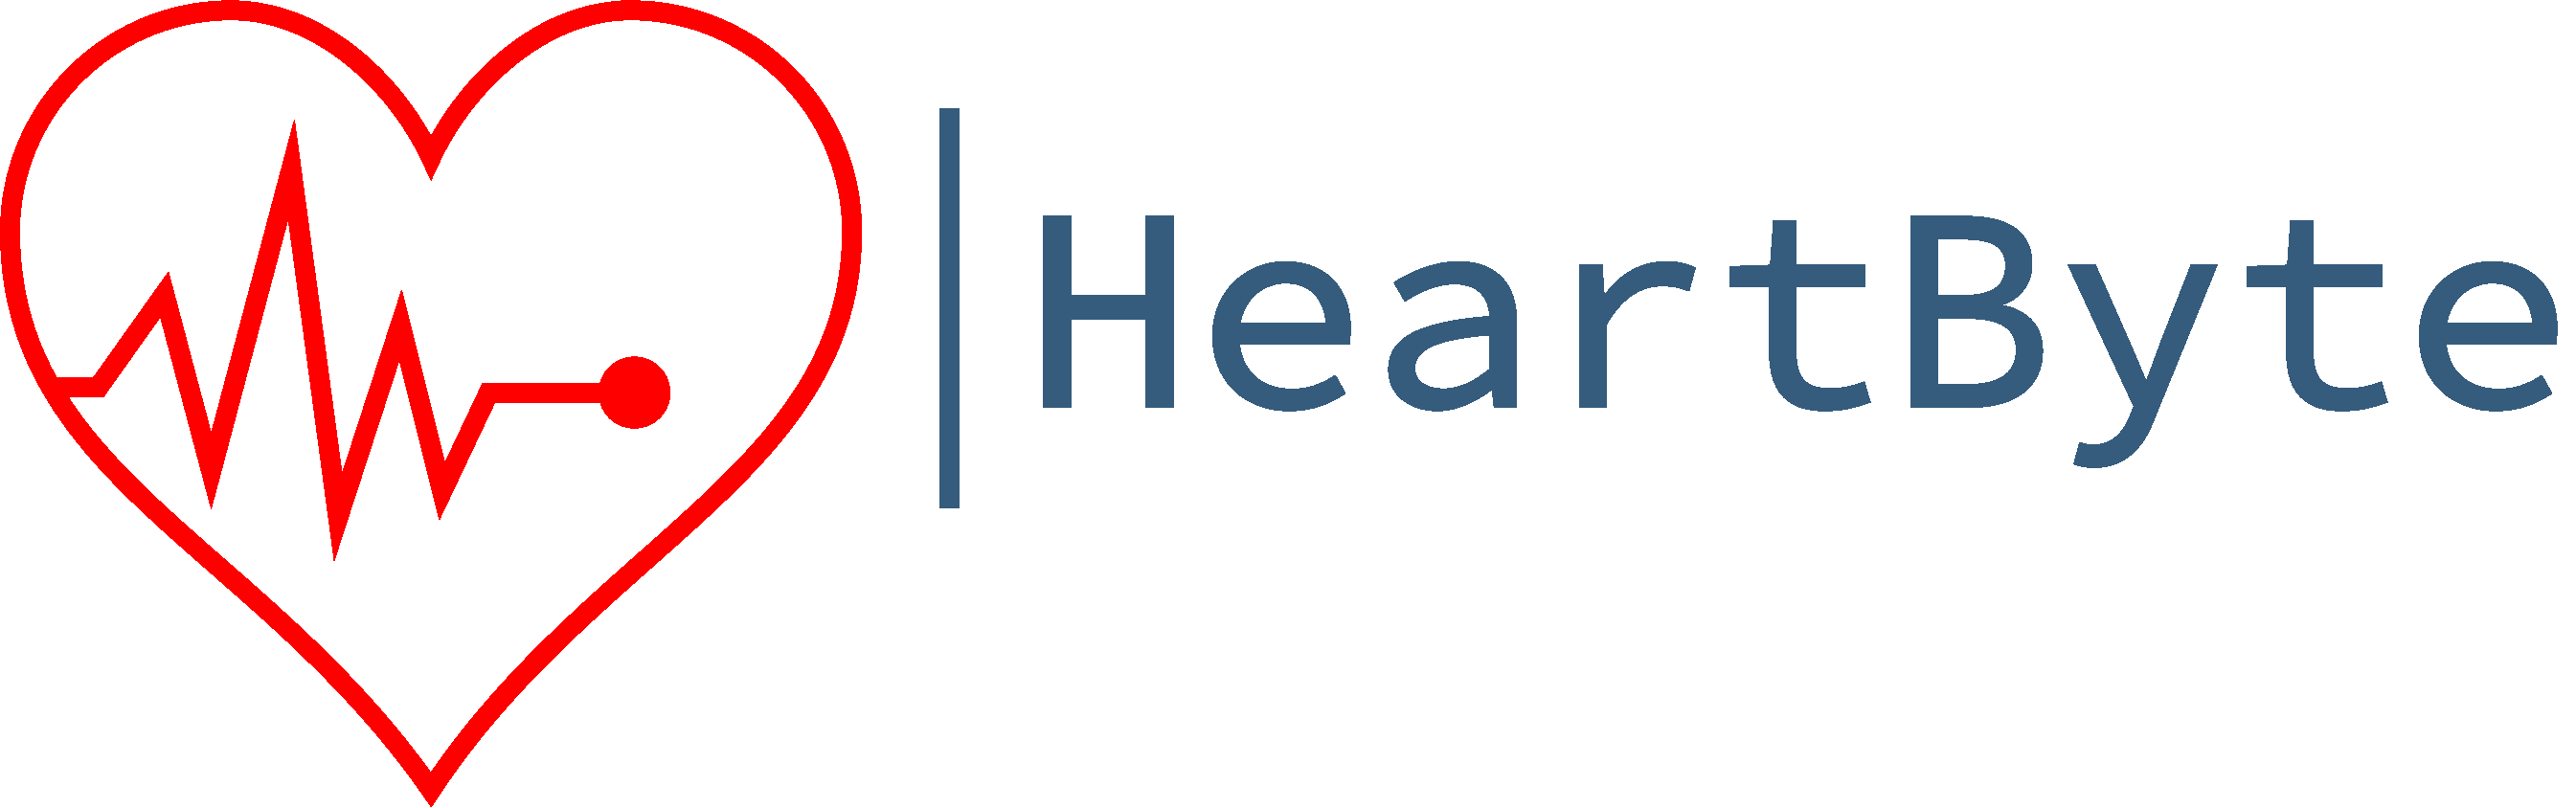
\includegraphics[width=\linewidth]{Pictures/logo_heartbyte_transparent_v_1_1 (1)}

    \vfill
            
   \end{center}
\end{titlepage}
\clearpage

% Workshops
    \section{Workshops}
  When development methods include new tools, we select someone responsible for the area who is supposed to gain a deeper understanding about the forementioned tool. The person mentioned is then in charge of making sure that the rest of the team that is supposed to work with the tool gains the required knowledge about it. This is done via workshops online where the responsible person goes through the basics of the tool.  A workshop could also include different brainstorming activities, where the participants are to come up with ideas regarding risks, company name, requirements for the system or tools to use for a specific system.
  
% Presentations
    \section{Presentations}
The management produces presentations to give during CEO meetings to educate the team in what has been done during the week and what is to be done during the upcoming weeks. The management is also supposed to highlight what in the process that is the most critical to get done as soon as possible. The presentations might also be used to educate the team in processes and tools that makes the work more effective. Example of tools that this may include is GitLab, Azure DevOps and different programming languages. The presentations could also be about how to handle documents and where to place documents for them to be easily found once they are needed. 

% Resource Sharing
    \section{Resource sharing}
 Through sharing resources in Teams and GitLab the team tries to share the knowledge and progression within their work. This assures that the whole team gets to take part of each other’s knowledge and where they currently are in terms of progression. It also prevents two people doing the same thing on different ends. 
 
% Group meeting & discussions
    \section{Group meetings and discussions}
The team is divided into different teams, both smaller cross-functional teams and teams where the whole group is working together on a specific task. The cross-functional teams makes it easier to share the information between the R&D department and the P&S department and makes sure that the information is shared and spread across the whole company. These group meetings are supposed to take place at least once every week.

%communication directives
    \section{Communication directives}
Through set up communication directives every person in the group should know who their main contact is for sharing the information that they want to spread or to gain the information that they want to acquire. A Communication structure has been set in order to make sure that a single person in the entire company talks with everyone else in the company since this can make the information that we are trying to be spread, get lost or be misinterpreted.    
\end{document}